\documentclass{report}
\usepackage[utf8]{inputenc}
\usepackage{xcolor}
\usepackage{sectsty} %%Pour changer la couleur de la police 
\usepackage{hyperref}
\usepackage{float}%%Pour les figures
\usepackage{listings}
\usepackage{amsmath}%%Pour les formules mathématique
\usepackage[final]{pdfpages}%%Pour l'inclusion de PDF
\usepackage{lscape}%%Pour passer une page en format paysage
\usepackage{graphicx}%%Pour rotation image
\usepackage{rotating}%%Pour rotation image

\title{Rapport}
\author{}
\date{}


\renewcommand{\contentsname}{Table des matières}
\renewcommand{\chaptername}{Chapitre}
\renewcommand{\appendixname}{Annexe}
\renewcommand{\bibname}{Bibliographie}

\definecolor{bleurapport}{HTML}{00AAD4}

\chapterfont{\color{bleurapport}}
\sectionfont{\color{bleurapport}}
\subsectionfont{\color{bleurapport}}

\begin{document}

\maketitle

\newpage
\null %%Pour faire une page vide
\newpage

\tableofcontents %%Table des matières
\newpage

\chapter{Introduction}
\section{Généralités}
\hspace{0.5cm}Alors qu'actuellement, de plus en plus de méthodes de profilage sont établies dans le monde des jeux afin de trouver le profil d'un joueur adverse, le poker est un jeu qui pose problème dans le domaine de l'intelligence artificielle. En effet, ce jeu est basé sur les connaissances de l'IA qui peuvent être erronées ou incomplètes, mais il existe aussi d'autres propriétés qui en font un jeu intéressant, comme la chance et le bluff. De ce fait, un joueur ne peut jamais être sûr à 100\% de pouvoir gagner et donc, son adversaire ne peut pas connaître de manière certaine le jeu qu'il peut avoir. C'est pourquoi dans ce type de jeu, le profilage est l'élément central du système d'intelligence artificielle. Cependant il est également difficile de profiler un joueur de manière certaine. Il y a donc des recherches dans le développement de méthodes permettant de profiler un joueur de manière efficace.\par

\section{Sujet}
\hspace{0.5cm}Le but de notre projet est de mettre en place le profilage d'un joueur de poker afin de déterminer de façon efficace le comportement de ce joueur. C'est à dire déterminer si le jouer est caractérisé comme agressif, passif, ou encore s'il a une tendance à bluffer.\par
Pour ce faire, nous devrons tout d'abord établir une méthode de profilage statique. C'est à dire, une technique pour profiler un joueur en fonction des actions qu'il a effectué pendant toute une partie, de manière globale. Après avoir implémenté cette première méthode de profilage, nous devrons mettre en place une intelligence artificielle pouvant jouer en fonction des résultats obtenus. Ainsi, nous pourrons voir si notre intelligence artificielle est capable de gagner plus de parties une fois le profil du joueur adverse établi.\par
S'il nous reste du temps, nous devrons mettre en place une méthode de profilage dynamique. Dans ce cas, il s'agit d'un profil qui s’établit tout au long de la partie et qui est modifié à chaque nouvelle action du joueur adverse. Nous devrons alors, de même que précédemment, mettre en place une intelligence artificielle capable de jouer en exploitant les données de profilage. Ainsi, nous pourrons observer la différence du nombre de parties gagnées en fonction des deux types de profilage, à savoir, statique ou dynamique, mais aussi en fonction des profils établis. En effet, un joueur considéré comme agressif et rationnel est-il plus facile à profiler et à battre qu'un joueur considéré comme non agressif et irrationnel ?\par

\chapter{Panification prévisionnelle}
\section{Analyse}
\hspace{0.5cm}Comme on peut le voir dans l'annexe A représentant le diagramme de Gantt prévisionnel du déroulement du projet, un premier jour sera accordé à une étude préalable durant laquelle les membres du groupe devront se familiariser avec les règles du poker et les termes techniques. De plus, durant cette période, les membres du groupe devront établir ensemble les normes de programmation qui seront respectées par la suite tout au long du projet.\par
Par la suite, notre projet sera divisé en quatre sous-projets. 
Le sous-projet correspondant à l'interface graphique commencera tout d'abord pendant une étude détaillée durant laquelle il faudra décider entre-autres des technologies à utiliser pour son développement. L'implémentation de l'interface graphique commencera ensuite, suivie par une série de tests visant à vérifier que l'interface graphique est bien fonctionnelle et répond aux besoins. \par
Dans le même temps, le sous-projet correspondant à la mise en place de l'intelligence artificielle basique et le jeu commencera. Celui-ci débutera d'abord par une étude préalable durant laquelle il faudra établir de façon claire et précise les différentes règles du Texas Hold'Em Poker. Une fois ces règles établies, une courte étude détaillée aura lieu, afin de discuter des différents points techniques de la mise en place du jeu et des différentes technologies qui pourraient être utilisées. Le jeu et l'intelligence artificielle seront alors développés puis testés.\par
Une fois les deux premiers sous-projets finis, le sous-projet "profilage statique" débutera. Le but de ce sous-projet sera de mettre en place des méthodes permettant de profiler de manière statique un joueur. Il commencera tout d'abord par une étude préalable durant laquelle une analyse de l'existant sera effectuée notamment par la lecture d'articles sur le sujet. Puis, une petite étude détaillée sera effectuée afin de bien définir les calculs qui seront à implémenter. La tâche de développement des algorithmes à implémenter commencera alors, avec l'écriture formelle des différents algorithmes de calculs qui devront être présents dans l'application. Enfin, l'implémentation des algorithmes dans l'application commencera, suivie par la phase de test des données ajoutées à l'application. \par
Enfin, le sous-projet "profilage dynamique" débutera. De même que pour le sous-projet "profilage statique", il débutera par une phase d'analyse de l'existant avec lecture d'articles traitant du sujet. Puis, sera suivi par une étude détaillée. Par la suite, une phase d'étude technique commencera avec le développement des algorithmes à implémenter. Enfin, les phase d'implémentation des algorithmes et de tests suivront.\par
En parallèle à toutes ses tâches aura lieu la rédaction du rapport et, à la fin du temps imparti, la préparation de la soutenance et de la démonstration. \par

\section{Méthode}
\subsection{Utilisation d'un gestionnaire de version}
\hspace{0.5cm}Afin de permettre un partage efficace des données, le gestionnaire de version Git sera utilisé. Le répertoire principal sera celui de Morgane Vidal \url{https://github.com/Gouga34/TERM1_Poker}, qui sera le responsable de l'intégration du projet. Les deux autres membres du projets Manuel Chataigner et Benjamin Commandre devront envoyer leurs ajouts sur leurs propres répertoires puis demander à ajouter leurs modifications sur le répertoire principal.\par

\chapter{Planification réelle}
\section{Comparaison entre le réel et le prévisionnel}
\hspace{0.5cm}Le diagramme de Gantt de l'annexe B correspond à la planification réelle de notre projet. Comme on peut vite le constater, nous avons eu du retard et n'avons pas pu finir toutes les tâches prévues au départ. De même, on peut constater que quelques tâches absentes au départ ont été ajoutées.\par

On peut tout d'abord voir que la mise en place de l'interface graphique a pris plus de temps que prévu. En effet, nous n'avions pas prévu que la bibliothèque que nous souhaitions utiliser s’avérerait difficile à mettre en place et que par conséquent il nous faudrait partir de zéro pour l'interface graphique. Étant donné le retard pris pour la mise en place de l'interface graphique, nous avons aussi pris quelques jours de retard sur l'implémentation du jeu de poker et de l'intelligence artificielle basique. \par
Cependant, on peut constater que nous avions commencé l'analyse de l'existant pour le profilage statique bien en avance. Cependant, nous avions ajouté à la liste des articles à lires quelques articles supplémentaires dont une thèse qui nous aura donc pris plus de temps à lire que précédemment. De ce fait, nous avons pris du retard sur la phase d'étude détaillée et sur la phase de développement des algorithmes. De plus, lorsque nous avons voulu passer à la phase d'implémentation des algorithmes. Nous devions récupérer une calculette de probabilités permettant de calculer les chances de gain d'un joueur. Cependant, cette calculette n'ayant pas été retrouvée, nous avons du ajouter de nouvelles tâches : l'étude détaillée et l'implémentation de la calculette de probabilité. Par conséquent, nous avons mis en pause l'implémentation des algorithmes afin que tous les membres du groupe puissent discuter ensemble de l'étude détaillée de la calculette de probabilités. De ce fait, nous avons pris encore plus de départ dans le déroulement de notre projet. \par

Comme on peut le constater, à mi-parcours du projet, du 31 mars au 10 avril, nous nous sommes rendus compte que la partie concernant le jeu et l'intelligence artificielle était difficilement réutilisable et que l'on découvrait régulièrement des bogues qui n'avaient pas été détectées au moment des tests. Cette partie étant difficilement débogable et nous faisant perdre beaucoup de temps, nous avons choisi de reprendre complètement cette partie. Nous avons perdu beaucoup de temps à ce moment là et nous nous sommes rendus compte à quel point la découverte tardive d'un bogue fait perdre énormément de temps sur le développement de l'application. Par conséquent, alors que la période d'implémentation des algorithmes liés au profilage statique aurait du être finie, nous avons repris le code du jeu et avons donc retardé cette implémentation, ce qui a fait prendre du retard aux tâches suivantes.\par

Enfin, nous pensions au départ que nous ne devrions que profiler les joueurs adverses alors que nous devions aussi faire jouer l'intelligence artificielle en fonction du profil établi afin de faire en sorte que l'intelligence artificielle gagne le plus d'argent possible. De ce fait, nous avons ajouté les tâches en rapport à la mise en place du jeu de l'intelligence artificielle en fonction des profils établis. \par

Nous pouvons donc en conclure que nous avons pris beaucoup de retard, sûrement à cause du fait que nous n'avions pas bien compris l'ampleur des tâches qui seraient à effectuer et à cause d'une mauvaise conception au départ de la partie correspondant au jeu et à l'intelligence artificielle basique. Finalement, étant donné que l'on s'est rendu compte du retard pris sur le projet, plutôt que terminer précipitamment la partie sur le profilage statique pour commencer le profilage dynamique prévu, nous avons préféré ne pas nous précipiter et terminer correctement le profilage statique et obtenir de bons résultats, quitte à ne pas faire la partie dynamique. \par


\section{Répartition des tâches}

		\begin{figure}[h]
			%\begin{center}
			\hspace{-3cm}\begin{tabular}{|l|l|l|}
				\hline
				Étude préalable & & \\
				\hline
  				 Interface Graphique & &  \\
  				 \hline
  				 & Étude Détaillée &  \textcolor{blue}{Manuel}  \textcolor{red}{Morgane}  \textcolor{purple}{Benjamin}\\
  				 \hline
  				 & Programmation & \textcolor{blue}{Manuel}\\
  				 \hline
  				 & Tests & \textcolor{blue}{Manuel}  \textcolor{red}{Morgane}\\
  				 \hline
  				 IA Basique & & \\
  				 \hline
  				 & Étude Préalable & \textcolor{blue}{Manuel}  \textcolor{red}{Morgane}  \textcolor{purple}{Benjamin}\\
  				 \hline
  				 & Étude Détaillée & \textcolor{purple}{Benjamin}\\
  				 \hline
  				 & Création IA (Programmation) & \textcolor{purple}{Benjamin}\\
  				 \hline
  				 & Tests & \textcolor{purple}{Benjamin} \textcolor{red}{Morgane}\\
  				 \hline
  				 Profilage Statique & &\\
  				 \hline
  				 & Analyse de l'existant & \textcolor{blue}{Manuel}  \textcolor{red}{Morgane} \\
  				 \hline
  				 & Étude détaillée & \textcolor{blue}{Manuel}  \textcolor{red}{Morgane}  \textcolor{purple}{Benjamin}\\
  				 \hline
  				 & Étude technique & \textcolor{blue}{Manuel}  \textcolor{red}{Morgane}  \textcolor{purple}{Benjamin}\\
  				 \hline
  				 & Implémentation Algorithmes & \textcolor{blue}{Manuel}  \textcolor{red}{Morgane}  \textcolor{purple}{Benjamin}\\
  				 \hline
  				 & Tests & \textcolor{blue}{Manuel}  \textcolor{red}{Morgane} \\
  				 \hline
  				 Jeu IA en fonction des résultats du profilage & &\\
  				 \hline
  				 & Étude Technique & \textcolor{blue}{Manuel}  \textcolor{red}{Morgane} \\
  				 \hline
  				 & Programmation & \textcolor{blue}{Manuel}  \textcolor{red}{Morgane} \\
  				 \hline
  				 Calculette de Probabilités & & \\
  				 \hline
  				 & Étude Détaillée & \textcolor{blue}{Manuel}  \textcolor{red}{Morgane} \textcolor{purple}{Benjamin}\\
  				 \hline
  				 & Implémentation Calculette de Probabilités & \textcolor{purple}{Benjamin}\\
  				 \hline
  				 & Implémentation Évaluateur de mains & \textcolor{red}{Morgane} \\
  				 \hline
  				 Rapport & & \textcolor{blue}{Manuel}  \textcolor{red}{Morgane} \\
  				 \hline
  				 Remaniement Jeu & & \textcolor{blue}{Manuel}  \textcolor{red}{Morgane} \\
   				\hline
			\end{tabular}	
			%\end{center}
			\caption{Répartition des tâches}
		\end{figure}
		\medskip

\hspace{0.5cm}Afin de travailler de manière efficace, nous avons choisi de nous répartir certaines tâches. Ainsi, nous avons tous participé à la première tâche, à savoir l'étude préalable. En effet, cette étape était essentielle à tout le monde puisque nous devions entre-autres maîtriser le sujet. Par la suite, pour les deux sous-projets concernant l'interface graphique et l'intelligence artificielle basique, tous les membres du groupe ont participé à l'étude détaillée de l'interface graphique ainsi qu'à l'étude préalable de l'intelligence artificielle. Ensuite, Manuel Chataigner a développé l'interface graphique pendant que Benjamin Commandré faisait la partie étude détaillée de l'intelligence artificielle et la développait. Morgane Vidal a ensuite effectué les tests de chacun des sous-projets cités précédemment. Par la suite, Manuel Chataigner et Morgane Vidal ont effectué l'analyse détaillée, en lisant plusieurs articles et en faisant leurs résumés. Chacun des membres du groupe ont ensuite participé à l'étude détaillée du profilage statique. \par
De même, comme on peut le voir dans le schéma ci-dessus, nous avons tous participé à l'étude technique du sous-projet profilage statique. En effet, les algorithmes à développer étant complexes, nous avons préféré être plusieurs pour en discuter et confronter nos points de vue. Nous avons donc développé ensemble durant cette tâche la méthode d'établissement du profil du joueur adverse. Puis, Manuel Chataigner et Morgane Vidal ont développé dans cette même tâche la méthode de calcul des scénarios de tests. Ensuite, chacun des membres du groupe ont participé à l'implémentation des algorithmes de calcul du profil basique du joueur adverse. Benjamin Commandré a implémenté l'utilisation des méthodes de calculs dans l'intelligence artificielle, Manuel Chataigner a implémenté l'écriture des résultats des profils établis dans un fichier de sortie, Morgane Vidal a implémenté les méthodes de calcul du profilage et Manuel Chataigner et Morgane Vidal ont implémenté l'utilisation des scénarios de tests. 
Par la suite, la phase de tests du profilage statique a été réalisée par Manuel Chataigner et Morgane Vidal. \par
Dans le sous-projet calculette de probabilités, nous avons tous participé à la tâche étude détaillée. Puis, Benjamin Commandré a implémenté la calculette de probabilités et Morgane Vidal a implémenté l'évaluateur de main.\par
La phase de reprise du code de la classe jeu, a été réalisée par Manuel Chataigner et Morgane Vidal. \par
Enfin l'écriture du rapport a été réalisée par Manuel Chataigner et Morgane Vidal.\par

\chapter{Données quantitatives}

\section{Organisation du travail}
\hspace{0.5cm}Comme prévu au départ, nos tuteurs et nous-même avons choisi de nous réunir chaque semaine afin de discuter de nos avancées, des éventuels problèmes rencontrés et des méthodes choisies pour le profilage. De ce fait, nous garantissions que ce que nous faisions était toujours en accord avec les attentes.\par
De notre côté, nous avions choisi de nous réunir chaque mercredi et chaque vendredi matin afin de pouvoir réfléchir ensemble sur les différentes méthodes de calculs. Par exemple, comment déterminer le taux d'agressivité d'un joueur ? Nous nous répartissions ensuite le contenu à implémenter.\par
Étant donné le fait que notre groupe n'était composé que de trois membres, nous avons choisi de ne pas élire de chef de projet mais plutôt de travailler tous sur un pied d'égalité. De ce fait, il n'y a pas eu de spécialisation, chaque membre du groupe a participé à toutes les parties du projet. En effet, notre projet étant basé en particulier sur la réflexion et sur la mise en place de différents algorithmes, il était plus intéressant de travailler à plusieurs.\par

\section{Mise en place de la méthode git-flow}
\hspace{0.5cm}Après avoir assisté au cour durant lequel les différentes architectures Git nous étaient présentés, nous avons choisi d'utiliser un git workflow pour la gestion de notre projet. Cette méthode consiste à mettre en place une branche master qui contient le code de production et sur laquelle rien n'est développé. Elle est donc réservée aux versions fonctionnelles et abouties.
Nous avons ensuite une branche develop sur laquelle sont ajoutées l'ensemble des modifications effectuées au cours du développement et le code qui sera ajouté pour la nouvelle release. Sur cette branche, on peut corriger ou encore améliorer des fonctions. \par
C'est donc une fois l'application dans une version finalisée que sont par la suite ajoutées à la branche master l'ensemble des commits effectués sur le develop.\par
Etant donné le fait que notre projet n'est pas un grand projet, et que nous ne sommes pas nombreux, nous avons choisi de ne pas mettre en place de branches feature, release et hot-fix. En effet, le temps de mettre en place une version de notre projet prend le temps imparti pour la mise en place du projet.\par
Pour chaque nouvelle fonctionnalité ou correction, nous ajoutions une nouvelle branche en local dans nos répertoires sur laquelle les modifications étaient effectuées. Elles étaient ensuite intégrées à la branche develop en local puis envoyées sur le répertoire public correspondant. Enfin, elles étaient intégrées au répertoire de référence.\par


\section{Brainstorming}
\hspace{0.5cm}Après avoir assisté au cour présentant les brainstorming, nous avons décidé d'en mettre en place un. En effet, nous étions à ce moment là du projet un peu perdu et ne savions plus que faire. Nous avions beaucoup de tâches à effectuer en même temps et ne savions pas par lesquelles commencer. Comme on peut le voir dans la figure suivante, nous avons donc mis sur papier chacune des tâches à effectuer puis, nous les avons classées par ordre de priorité et partagées entre les différents membres du groupe. \par
%%TODO : mettre une des photos du brain storming%%


\section{Quelques chiffres}
\hspace{0.5cm}La figure suivante représente la courbe des commits effectués par tous les membres du groupe. Comme on peut le voir, nous avons tous plus ou moins participé. De plus, nous pouvons voir sur cette figure que chacun des membres a ajouté un certain nombre de lignes de code au projet. Le fort nombre de lignes supprimées pour Manuel Chataigner et Morgane Vidal est dû au remaniement de la classe jeu ainsi qu'à la mise en ligne du rapport et des différents commits en rapport.\par

%%%%%%%%%%%%%%%%%%%%%%%%%%%%%%%%%%%%%%%%%%%%%%%%%%%%%%%%%%%%%%%%%%%%%%%%%%%%%%%%%%%%%%%%%
%%%%%TODO mettre un screenshot de la courbe des commits %%%%%%%%%%%%%%%%%%%%%%%%%%%%%%%%%
%%%%%%%%%%%%%%%%%%%%%%%%%%%%%%%%%%%%%%%%%%%%%%%%%%%%%%%%%%%%%%%%%%%%%%%%%%%%%%%%%%%%%%%%%



%% Retour sur le comparatif, explication des modifications.
%%%git, nb commits / codes ...
%% CMMI MA
%% lien entre III et IV

\chapter{Conclusion}

\hspace{0.5cm}La mise en place de ce projet nous a fait découvrir à quel point plus la détection d'un bogue est tardive, plus on perd du temps. En effet, nous avons perdu beaucoup de temps à remanier les classe jeu et intelligence artificielle car celles-ci étaient mal conçues et nous perdions beaucoup de temps à chaque découverte de bogue, dont certains étaient découverts plusieurs semaines après la fin de la phase de tests de cette partie. \par
Durant se projet, nous avons choisi d'utiliser dès que possible les méthodes vues au fur et à mesure en cours. De ce fait, après avoir découvert l'utilisation des workflow, nous avons modifié l'architecture de notre Git pour passer en git-flow. De même, après avoir découvert les méthodes agiles et notamment d'utilisation du brainstorming pour faire sortir de manière efficace un maximum d'idées et de tâches à effectuer. \par

\appendix
\chapter{Diagramme de Gantt prévisionnel}
	\begin{sidewaysfigure}[ht]
		 \hspace{-4cm} 
			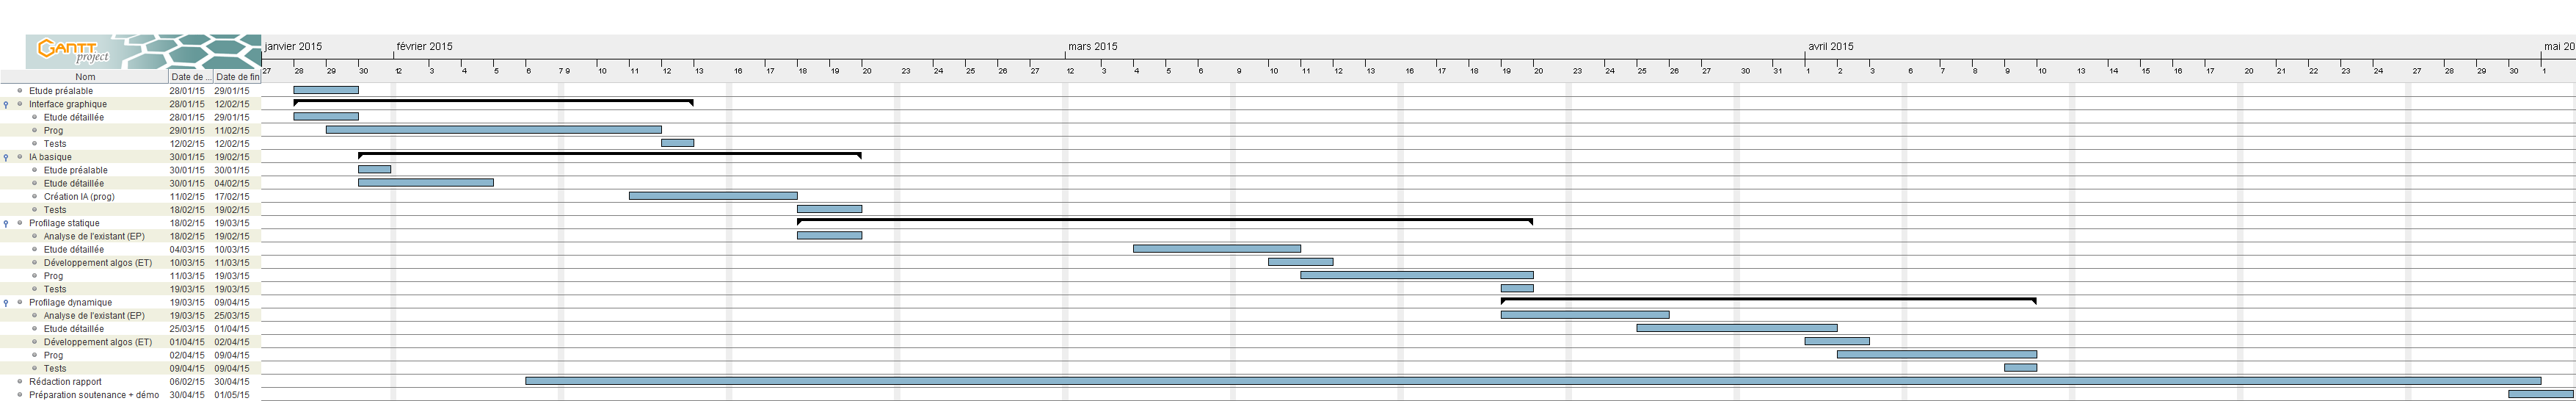
\includegraphics[scale=0.3]{../DiagrammePrevisionnel.png}
			\caption[Planification Prévisionnelle]{Planification Prévisionnelle}
	\end{sidewaysfigure}
	\medskip


\chapter{Diagramme de Gantt réel}
	\begin{sidewaysfigure}[ht]
		 \hspace{-4cm} 
			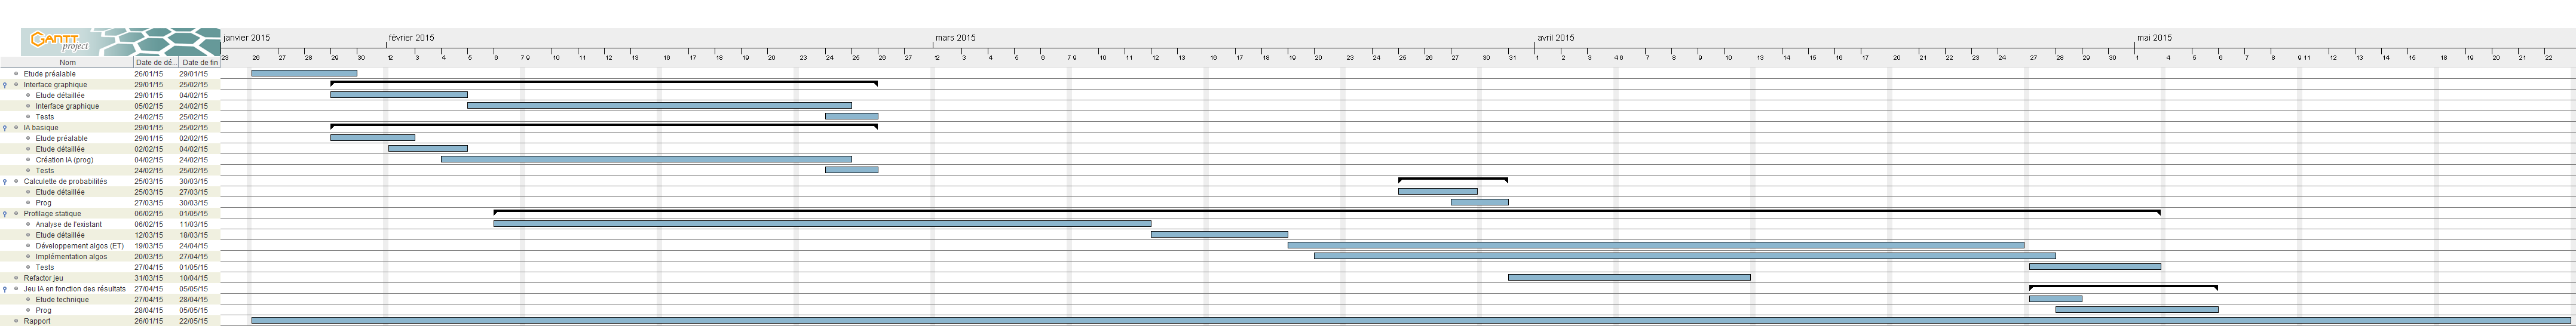
\includegraphics[scale=0.3]{../DiagrammeReel.png}
			\caption[Planification réelle]{Planification réelle}
	\end{sidewaysfigure}
	\medskip

\end{document}